\begin{figure}[H]
    \centering
    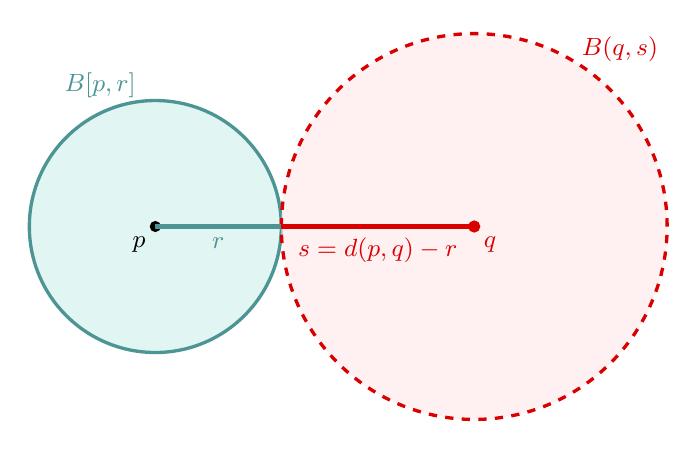
\begin{tikzpicture}[scale=1.0, every node/.style={font=\small}]
        \coordinate (p) at (0,0);
        \coordinate (a) at (1.6,0);
        \coordinate (q) at (4.05,0);

        % Bola fechada B[p,r].
        \path[fill=BlueGreen!14] (p) circle (1.6);
        \draw[BlueGreen!70!black, very thick] (p) circle (1.6);
        \node[BlueGreen!70!black] at (-0.7,1.8) {$B[p,r]$};

        % Bola aberta centrada em q.
        \path[fill=Red!8, fill opacity=0.72] (q) circle (2.45);
        \draw[Red!85!black, very thick, dashed] (q) circle (2.45);
        \node[Red!85!black] at (5.9,2.25) {$B(q,s)$};

        % Pontos principais.
        \filldraw[black] (p) circle (1.8pt) node[below left] {$p$};
        \filldraw[Red!85!black] (q) circle (2pt) node[below right] {$q$};

        % Distancias relevantes.
        \draw[BlueGreen!70!black, ultra thick] (p) -- (a)
            node[midway, below] {$r$};
        \draw[Red!85!black, ultra thick] (a) -- (q)
            node[midway, below] {$s=d(p,q)-r$};
    \end{tikzpicture}
    \caption{A bola aberta de centro $q$ e raio $s=d(p,q)-r$.}
    \label{fig:bolaFechadaFechado}
\end{figure}
